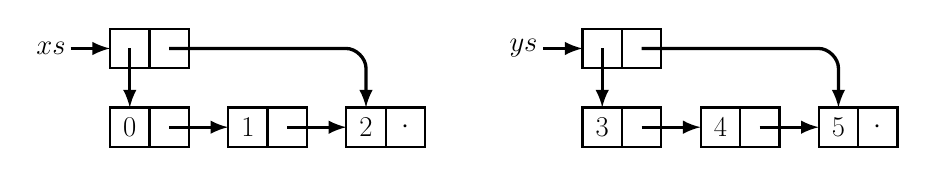
\begin{tikzpicture}[thick,scale=0.5, every node/.style={scale=0.5}]
    \tikzstyle{marrs}=[very thick,-latex]

    \begin{scope}
    
        \foreach \x/\y in {0/0, 0/-2, 3/-2, 6/-2} {
            \draw (\x - 0.5, \y - 0.5) rectangle +(1, 1); \draw (\x + 1 - 0.5, \y - 0.5) rectangle +(1, 1);
        }
        \draw[marrs] (-1.5, 0) -> +(1, 0);
        \draw[marrs] (0, 0) -> +(0, -1.5);
        \draw[marrs] (1, -2) -> +(1.5, 0);
        \draw[marrs] (4, -2) -> +(1.5, 0);
        \draw[marrs] (1, 0) -- (5.5, 0) .. controls (5.75, 0) and (6, -0.25) .. (6, -0.5) -- (6, -1.5);
        
        { \huge
            \draw (-2, 0) node {$xs$};
            \draw (0, -2) node {$0$};
            \draw (3, -2) node {$1$};
            \draw (6, -2) node {$2$};
            \draw (7, -2) node {$\cdot$};
        }
    
    \end{scope}
    
    \begin{scope}[xshift=12cm]
    
        \foreach \x/\y in {0/0, 0/-2, 3/-2, 6/-2} {
            \draw (\x - 0.5, \y - 0.5) rectangle +(1, 1); \draw (\x + 1 - 0.5, \y - 0.5) rectangle +(1, 1);
        }
        \draw[marrs] (-1.5, 0) -> +(1, 0);
        \draw[marrs] (0, 0) -> +(0, -1.5);
        \draw[marrs] (1, -2) -> +(1.5, 0);
        \draw[marrs] (4, -2) -> +(1.5, 0);
        \draw[marrs] (1, 0) -- (5.5, 0) .. controls (5.75, 0) and (6, -0.25) .. (6, -0.5) -- (6, -1.5);
        
        { \huge
            \draw (-2, 0) node {$ys$};
            \draw (0, -2) node {$3$};
            \draw (3, -2) node {$4$};
            \draw (6, -2) node {$5$};
            \draw (7, -2) node {$\cdot$};
        }
    \end{scope}
    
    
    
\end{tikzpicture}